
%%%%%%%%%%%%%%%%%%%%%%%%%%%%%%%%%%%%%%%%%%%%%%%%%%%%%%%%%%%%%%%%%%%%%
%% This is a (brief) model paper using the achemso class
%% The document class accepts keyval options, which should include
%% the target journal and optionally the manuscript type.
%%%%%%%%%%%%%%%%%%%%%%%%%%%%%%%%%%%%%%%%%%%%%%%%%%%%%%%%%%%%%%%%%%%%%
\documentclass[journal=jacsat,manuscript=article]{achemso}

%%%%%%%%%%%%%%%%%%%%%%%%%%%%%%%%%%%%%%%%%%%%%%%%%%%%%%%%%%%%%%%%%%%%%
%% Place any additional packages needed here.  Only include packages
%% which are essential, to avoid problems later. Do NOT use any
%% packages which require e-TeX (for example etoolbox): the e-TeX
%% extensions are not currently available on the ACS conversion
%% servers.
%%%%%%%%%%%%%%%%%%%%%%%%%%%%%%%%%%%%%%%%%%%%%%%%%%%%%%%%%%%%%%%%%%%%%
\usepackage[version=3]{mhchem} % Formula subscripts using \ce{}
\usepackage[T1]{fontenc}       % Use modern font encodings

%%%%%%%%%%%%%%%%%%%%%%%%%%%%%%%%%%%%%%%%%%%%%%%%%%%%%%%%%%%%%%%%%%%%%
%% If issues arise when submitting your manuscript, you may want to
%% un-comment the next line.  This provides information on the
%% version of every file you have used.
%%%%%%%%%%%%%%%%%%%%%%%%%%%%%%%%%%%%%%%%%%%%%%%%%%%%%%%%%%%%%%%%%%%%%
%%\listfiles

%%%%%%%%%%%%%%%%%%%%%%%%%%%%%%%%%%%%%%%%%%%%%%%%%%%%%%%%%%%%%%%%%%%%%
%% Place any additional macros here.  Please use \newcommand* where
%% possible, and avoid layout-changing macros (which are not used
%% when typesetting).
%%%%%%%%%%%%%%%%%%%%%%%%%%%%%%%%%%%%%%%%%%%%%%%%%%%%%%%%%%%%%%%%%%%%%
\newcommand*\mycommand[1]{\texttt{\emph{#1}}}

%%%%%%%%%%%%%%%%%%%%%%%%%%%%%%%%%%%%%%%%%%%%%%%%%%%%%%%%%%%%%%%%%%%%%
%% Meta-data block
%% ---------------
%% Each author should be given as a separate \author command.
%%
%% Corresponding authors should have an e-mail given after the author
%% name as an \email command. Phone and fax numbers can be given
%% using \phone and \fax, respectively; this information is optional.
%%
%% The affiliation of authors is given after the authors; each
%% \affiliation command applies to all preceding authors not already
%% assigned an affiliation.
%%
%% The affiliation takes an option argument for the short name.  This
%% will typically be something like "University of Somewhere".
%%
%% The \altaffiliation macro should be used for new address, etc.
%% On the other hand, \alsoaffiliation is used on a per author basis
%% when authors are associated with multiple institutions.
%%%%%%%%%%%%%%%%%%%%%%%%%%%%%%%%%%%%%%%%%%%%%%%%%%%%%%%%%%%%%%%%%%%%%
\author{Robert O. Ness}
\email{nessr@purdue.edu}
\affiliation[Purdue University]{Department of Statistics, Purdue University, West Lafayette}
\author{Karen Sachs}
\affiliation[Stanford University]{School of Medicine, Stanford University, Palo Alto}
\email{karens1@stanford.edu}
\author{Olga Vitek}
\email{o.vitek@neu.edu}
\affiliation[Northeastern University]{College of Science, College of Computer and Information Science, Northeastern University, Palo Alto}


%%%%%%%%%%%%%%%%%%%%%%%%%%%%%%%%%%%%%%%%%%%%%%%%%%%%%%%%%%%%%%%%%%%%%
%% The document title should be given as usual. Some journals require
%% a running title from the author: this should be supplied as an
%% optional argument to \title.
%%%%%%%%%%%%%%%%%%%%%%%%%%%%%%%%%%%%%%%%%%%%%%%%%%%%%%%%%%%%%%%%%%%%%
\title[]
  {From Correlation to Causality: Statistical approaches to learning regulatory relationships from Large-scale Omics Experiments}

%%%%%%%%%%%%%%%%%%%%%%%%%%%%%%%%%%%%%%%%%%%%%%%%%%%%%%%%%%%%%%%%%%%%%
%% Some journals require a list of abbreviations or keywords to be
%% supplied. These should be set up here, and will be printed after
%% the title and author information, if needed.
%%%%%%%%%%%%%%%%%%%%%%%%%%%%%%%%%%%%%%%%%%%%%%%%%%%%%%%%%%%%%%%%%%%%%
\abbreviations{IR,NMR,UV}
\keywords{American Chemical Society, \LaTeX}

%%%%%%%%%%%%%%%%%%%%%%%%%%%%%%%%%%%%%%%%%%%%%%%%%%%%%%%%%%%%%%%%%%%%%
%% The manuscript does not need to include \maketitle, which is
%% executed automatically.
%%%%%%%%%%%%%%%%%%%%%%%%%%%%%%%%%%%%%%%%%%%%%%%%%%%%%%%%%%%%%%%%%%%%%
\begin{document}


%%%%%%%%%%%%%%%%%%%%%%%%%%%%%%%%%%%%%%%%%%%%%%%%%%%%%%%%%%%%%%%%%%%%%
%% Start the main part of the manuscript here.
%%%%%%%%%%%%%%%%%%%%%%%%%%%%%%%%%%%%%%%%%%%%%%%%%%%%%%%%%%%%%%%%%%%%%
\section{Introduction}
Causal inference -- the task of uncovering regulatory relationships
between components of biomolecular pathways and networks - is a primary
goal of omics datasets in molecular biology studies. Statistical
associations can reveal an alluring set of putative causal interactions,
but when are such associations significant and reliable? And when can
they be interpreted as causal? Our goal below is to provide suggestions
for causal inference in large scale experiments, such as those resulting
from high throughput omics technologies. We describe the pitfalls of
large datasets, and suggest methods to reliably find causal associations
despite these pitfalls.

High-throughput omics technologies enable large-scale experiments, with
simultaneous measurements of multiple cellular components in a sample.
The huge amount of data generated paradoxically make the task of causal
inference much more difficult, because, when many associations are
examined, some will appear significant just by chance. In other words,
large-scale experiments are more prone to hiding the true signal and
generating spurious associations, leading to increased false positive
conclusions that causal relationships are present. This problem can be
addressed by improving experimental design and/or refining the
biological question. Below, we describe the process of elucidating
statistical associations from data and suggest practical approaches for
analysis of large scale datasets.

\section{Discussion}
\subsection{I. Statistical inference of causal relationships}

In MAPK signaling, Raf causally affects active Mek levels (via
phosphorylation), while Mek causally affects Erk. Imagine this
relationship was unknown: could it be detected from measurements of
these phosphoproteins? Given sufficient data, a correlation will be
detected between each pair of proteins, due to (direct and indirect)
causal relationships. Figure 1, top panel, depicts these correlations as
black lines, causal relationships are depicted as blue arrows.

To go from correlation to causality, we need to perform an intervention:
for instance, we can use a small molecule inhibitor to block Mek
activity. Resulting measurements show an impact on Erk but not on Raf,
correctly orienting the two edges. Note that it was not necessary to
intervene on each node in order to get the correct causal directions,
from Raf to Mek and Mek to Erk. What about the noncausal edge? The edge
linking Raf to Erk is not causal, because Raf's effect on Erk occurs
only via Mek (and that affect is already represented, rendering the
Raf-Erk edge superfluous). In statistical inference, this edge can be
eliminated without the need of further interventions. How is this done?

First, some terminology. A statistical association (such as a
correlation) between two variables indicates that they are dependent.
Sometimes we choose to assess a dependence in the context of the value
of other system components, such as a third variable. In this case the
dependence is called conditional dependence, because it is evaluated
conditional on the state of other system components (i.e., the third
variable). Let's see how this applies here, by examining the dependence
between Raf and Erk. If we condition on Mek, then we assume that we know
the value of Mek: perhaps we limit our analysis to samples which have a high level
of Mek, so Mek is fixed at level "high". Can the dependence between
Raf and Erk still be detected? If, due to noise, some of these Mek=high
samples have an intermediate or even low level of Raf, will Erk be
correspondingly low? Based on the causal mechanism, Erk will more
closely follow Mek (i.e. its values will tend to be high), since Mek is 
its causal parent. Because of that, the Raf-Erk dependence, once conditioned 
on Mek, will be reduced or eliminated, thus indicating that the Raf-Erk edge 
can be removed. Using this approach, it is possible to keep only the causal edges 
as depicted by the black lines in Figure 1, bottom panel.

Computational methods for causal inference in the context of
experiments that simultaneously measure multiple intercorrelated
features all rely on finding conditional dependence.  All of these algorithms
essentially have the same two step process; (1)
reduce the dense set of pairwise associations to a sparse set of
conditional dependencies, (2) use information about the interventions
included in the experiment to evaluate those conditional dependencies as
evidence for potential causal relations.


\subsection{II. Inference with large numbers of variables}


Suppose we perform a large scale experiment, quantifying several
thousands of phosphoproteins, including Raf, Mek and Erk. A typical
large-scale experiments includes a very small number of interventions,
and around 3 replicates. Statistical inference fails in this case,
because the large number of variables measured result in a large number
of spurious statistical associations, which appear as strong as true
associations. The relationship between Raf, Mek and Erk, for instance,
will be obscured by the many spurious relationships that they will each
form with causally unrelated proteins.

\begin{figure}[!tpb]
\centerline{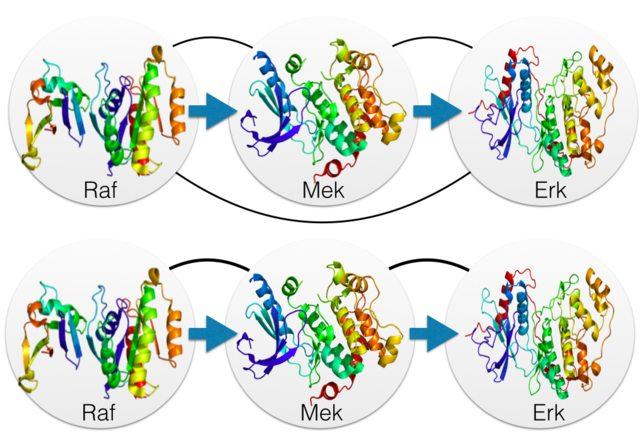
\includegraphics[width=0.5\textwidth]{figs/mapk.jpg}}
\caption{In the MAPK signaling pathway, Raf regulates Mek, which regulates
Erk. Top; the lines represent association - the activity of the kinases
on this pathway are all correlated. Bottom: the lines represent
conditional dependence, there is no conditional dependence edge from Raf
to Erk because given you know Mek, knowing Raf tells you nothing about
Erk. They are conditionally independent.}
\label{mapk}
\end{figure}

The problem of doing causal inference with large-scale experiments is
two-fold. Firstly, sample size is typically far too small for the large
number of features we measure. With the large-scale experiment described
above, it is clear that viewing a scatter-plot between a pair of
features that has only 3 points is uninformative -- even if the points
correlated perfectly, 3 points is not enough to conclude anything about
the relationship with any confidence. But even with hundreds of samples,
we are still plagued by spurious associations when the number of
features is so large, since more features means greater chance
associations will occur at random.

To illustrate, we ran a simulation where we first simulate a 20 features
dataset each with a 100 Gaussian random measurements, then increase the
number of features to 500. In both cases the features are completely
independent. This means if we quantify association using Pearson
correlation, any correlation we find will be completely spurious. We
record the maximum correlation between the 20 feature set and the 500
feature set. We repeat this simulation 500 times.

\begin{figure}[!tpb]
\centerline{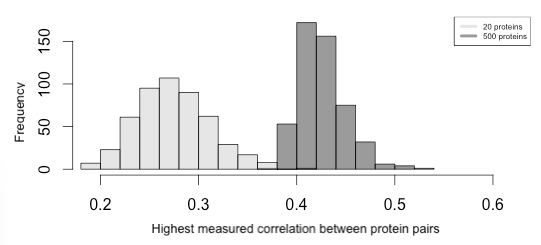
\includegraphics[width=0.5\textwidth]{figs/spurious_corr.png}}
\caption{Increasing the number of features results in more high scoring
spurious correlations.}
\label{spur_corr}
\end{figure}

The increased incidence of spurious correlation means increased false
positives in detecting conditional dependence relationships. To
illustrate, we repeat the previous simulation, except now expanding from
20 to only 100 features. In each of the 500 instances, we apply a search
algorithm that iteratively performs conditional independence tests,
returning a count of detected conditional dependence relationships. As
before, since we simulated independent features, any conditional
dependence relationship reported by this algorithm is a false positive,
i.e.~it doesn't actually exist in the mechanism that generated the data.

\begin{figure}[!tpb]
\centerline{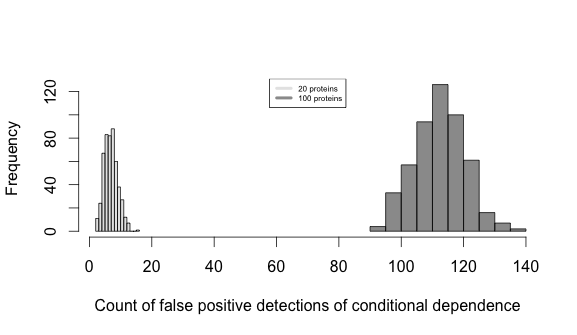
\includegraphics[width=0.5\textwidth]{figs/spurious_dep.png}}
\caption{Fig3. Increasing the number of measured features means increasing the
false positive detection of conditional dependence.}
\label{spur_dep}
\end{figure}

As we increased the number of features we measured, we saw a comparable increase in 
the number of false positive detection of conditional dependence relationships. What this
means is that the computational methods for causal inference will fail for the
typical large-scale experiment, because when their input data contains a
large amount of features relative to sample size, they cannot reliably
detect the conditional dependence relationships they need to infer
causality.

The second problem is the requirement for interventions. This is just as important as the 
problem of spurious conditional dependence, but much easier to explain -- as the number
of features grows, the number of interventions needed to infer causality
grows, and performing sufficient perturbation experiments becomes
infeasible.


\subsection{III. Inferring causality from omics experiments}

The problems outlined in section II paint a grim picture for causal
learning in large datasets. Fortunately, these can be overcome, and
effective causal learning can be a reality for large scale datasets. We
proffer the approaches listed in \textit{The Causality Inference in Omics Tool List}
below.

\begin{enumerate}
\item \textit{Refine the biological problem}, thus limiting the number of features. If
the broader biological system is well-studied, it may be possible design
an experiment that focuses on a specific part of the system of interest,
then ask more specific questions of the data, such as whether a
particular edge or pathway is present. The more specific the question,
the less data is needed overall to make solid statistical inferences.
\item \textit{Measure more samples}. If feasible, high throughput measurements that
measure many samples (not just many features) provide the statistical
power to tell true associations from spurious associations. This
intuition motivates the use technologies that have lower throughput but
enable measurement of more samples (or gather more data points per
sample), for causal modeling. An example is single cell mass cytometry,
where many thousands of cells per sample provide ample statistical
power.
\item \textit{Use prior knowledge}, not just from experts but also from noisier
sources, to improve the process of searching for conditional
independence. The MAPK pathway for instance, mentioned earlier, is well
established and canonical. Assuming it, and other well established
connections are present in the data a priori can help reduce the number of possible
associations, and enable more effective use of data. Knowledge about
canonical causal relationships can be sourced from pathway databases
such as KEGG. Another example is contextual information, such as spatial
relations between phosphoproteins in the cell -- causal inference
algorithms can be formulated to weigh evidence of conditional dependence
differently depending on whether phosphoproteins are from the same or
different spatial compartments. Employing prior knowledge that provides
evidence for the regulatory network reduces the number of connections
and causal arcs under consideration, which allows the available data to
make reliable statistical inferences.
\item \textit{Employ targeted interventions selectively}. Targeted interventions
perturb individual components of the system. An example is small
molecule inhibitors which block the causal influence of a specific
phoshoprotein on downstream components. Since it is usually prohibitive
to perturb every target component of a system, it is strategic to
prioritize application of targeted interventions to parts of the system
that have the most potential for new discoveries. Selection of these
perturbation targets can be based on prior knowledge - e.g.~knowledge of
which components are crucial players in the system of interest - or they
can be applied iteratively, after an initial statistical analysis has
revealed areas of the network in which causal inferences are not
possible based on existing data. For instance, a resulting model graph
with undirected edges can be inspected to reveal which nodes have
potential to reveal the most causality if perturbed.
\item \textit{Consider broad-scale interventions}. Traditionally, experiments consider
a biological response to a particular stimulus, possibly in the context
of an inhibitor. In contrast, broad-scale interventions sacrifice
specificity to perturb many features in the system simultaneously. The
advantage of this approach is that it can enable elucidation of
causality across the entire system. Just as one intervention was
sufficient to infer causality between 3 proteins Raf, Mek, and Erk,
perturbing many things at once creates cascades of causal direction
orientation across the broader network. This includes varying
experimental conditions to activate multiple pathways. For example,
signals from endocrine, paracrine, and autocrine ligands elicit various
signaling responses in hepatocytes, thus interventions that cover this
range of signals gives the best picture of the broader causal network of
hepatocyte signaling. Similarly, interventions that go beyond
receptor-level and perturb multiple components of the system bring
cascading causal direct orientation deeper into the network. In contrast
to targeted interventions, while it is difficult to know in advance what
information will provided by broad-scale interventions, they provide
more causal inference bang for your intervention buck.
\end{enumerate}

\textit{The Causality in Omics Tool List} above provides impactful approaches
that can drastically improve causal inference from omics datasets, by
constraining the inference task, and thus allowing for accurate
statistical inferences. For instance, the task of assessing which of all
the possible KEGG pathways is present in a dataset will be far less
error-prone than the task of assessing which of all possible
combinations of my measured features might form a biological pathway.

How should the tools listed be used? They are most powerful when used in
combination, and in fact the lines between them are somewhat arbitrary
and frequently blurred. For instance, using tool \#1 and tool \#2 in
concert can be thought of as reducing the breadth and increasing the
depth of the investigation. Tools \#4 and \#5 call for use of
interventions, but this task itself is complicated by measuring many
things, since we have more features to expose to intervention. Tool
\#3, prior biological knowledge, can be used to prioritize what to
target with that limited set of interventions.

\end{document}
